% Chapter Template

\chapter{Especificació} % Main chapter title

\label{Chapter5} % Change X to a consecutive number; for referencing this chapter elsewhere, use \ref{ChapterX}

Després d'haver explicat l'origen de \textit{Wisebite}, haver estudiat les solucions actuals del mercat i suggerit una de millor i haver analitzat els requisits i les funcionalitats del sistema, cal especificar els models que representaran les entitats que formaran el projecte. En primera instància, es mostrarà l'esquema conceptual que defineix el treball i s'explicarà cada una de les entitats que l'engloben. Per altra banda, s'analitzarà l'esquema de comportament que interacciona entre l'usuari i el sistema.

%----------------------------------------------------------------------------------------
%	SECTION 1
%----------------------------------------------------------------------------------------

\section{Esquema conceptual}

L'esquema conceptual d'un sistema és la representació gràfica dels models que caracteritzen aquest. En Enginyeria del Software això és conegut com un diagrama de classes\cite{diagramaclases}. Primerament, s'expressarà en format UML i posteriorment s'explicarà textualment.

\begin{figure}[!h]
\centering
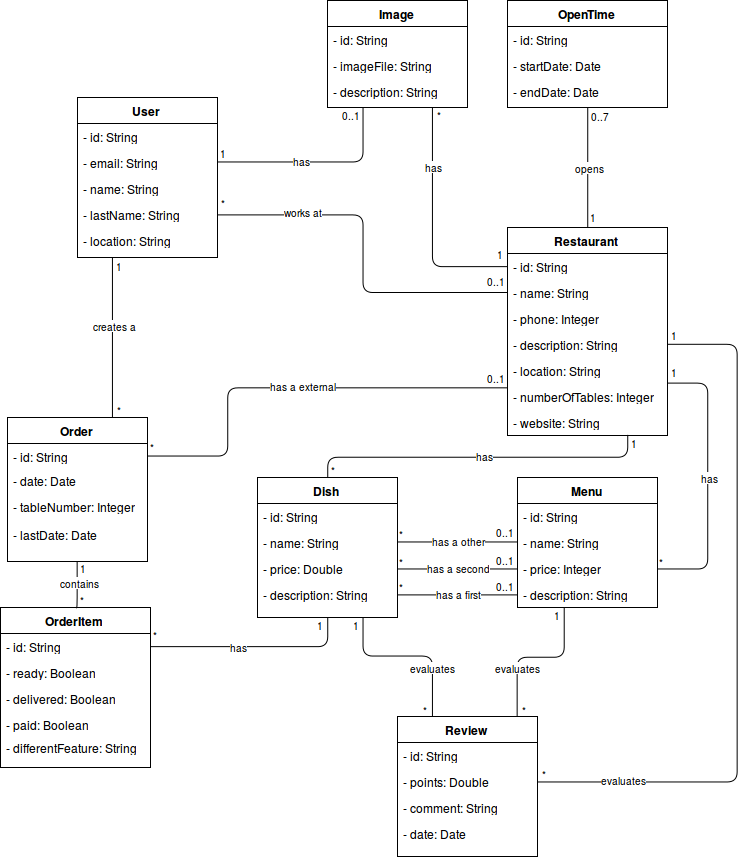
\includegraphics[scale=0.5]{Figures/diagrama_clases.png}
\caption{Diagrama de classes}
\end{figure}

%----------------------------------------------------------------------------------------
%	SECTION 2
%----------------------------------------------------------------------------------------

\clearpage
\section{Esquema del comportament}

TODO: Redactar